\documentclass{article}
\usepackage[options]{authblk}
\usepackage{graphicx} % Required for inserting images
\usepackage[utf8]{inputenc}
\usepackage[T2A]{fontenc}
\usepackage{hyperref}
%\usepackage{float}%Плавающие" картинки
\usepackage{wrapfig}%Обтекание фигур (таблиц, картинок и прочего)
\usepackage{multicol}


\title{Лабораторная работа по дисциплине "Теория функций комплексной переменной"}
\author{Горюнов Семён Олегович P3230, \and Захарченко Роман Владимирович P3231, \and Милёхина Елизавета Алексеевна P3232}
\date{October 2024}

\begin{document}

\maketitle

\section{Доказательство свойств множества Мандельброта}
\par \textit{Свойство 1.} Множество Мандельброта переходит само в себя при сопряжении.
\par Пусть c принадлежит множеству Мандельброта (c = x + iy).
\par Рассмотрим $\widetilde{z_{n+1}} = \widetilde{z_{n}}  + \bar c$. 
Докажем, что $\widetilde{z_{n}}$ сопряжено с ${z_{n}}$ по индукции.
\par База. n = 0.
$\widetilde{z_{0}}$ = $\bar{z_{0}}$
\par Переход от n к n+1. $\widetilde{z_{n}}$ = $\bar{z_{n}}$
\par $\widetilde{z_{n+1}}$ = $\widetilde{z_{n}}^2 + \bar c$ = $\bar{z_{n}}^2 + \bar c$ = $\bar{z_{n}^2} + \bar c$ = $\overline{z_{n}^2 + c}$
\par Следовательно, $\bar c$ принадлежит множеству Мандельброта.
\newline
\par \textit{Свойство 2.} Если |c| > 2, то c не принадлежит множеству Мандельброта.
\par Пусть |c| > 2. |c| = r = $1 + k$, r, k - действительный числа ($1 + k > 2$, следовательно $k > 1$).
\par Докажем, что $z_{n}$ не ограничено. Воспользуемся индукцией.
\par База: $|z_{0}| = 0$, $|z_{1}| = r$,  $|z_{2}| = |z_{1}^2 + c| \ge |z_{1}^2| - |c| = r^2 - r = r(r-1) = rk = rk^{2^{n-2}}$
\par Переход от n к n+1. $|z_{n+1}| = |z_{n} + c| \ge |z_{n}^2| - |c|$
\par $|z_{n}^2| - |c| = (rk^{2^{n-2}})^2 - r = r(rk^{2^{n-1}} - 1) = r(k^{2^{n-1}} + k^{2^{n-1}+1} - 1) \ge rk^{2^{n-1}}$. Так как k > 1, $k^{2^{n-1}+1} - 1 > 0$.
\par $|z_{n+1}| \ge rk^{2^{n+1}-2}$. Следовательно, т.к. k > 1, то $rk^{2^{n-1}}$ возрастает. Получаем, что $z_{n}$ не ограничено.
\section{Код для визуализации множества Мандельброта, Жюлиа и бассейнов Ньютона}
\url{https://github.com/dfa-ra/FractalsTFCV/tree/master}
\section{Немного о бассейнах Ньютона}
Еще один тип динамических фракталов составляют фракталы (так называемые бассейны) Ньютона. Формулы для их построения основаны на методе решения нелинейных уравнений, который был придуман великим математиком еще в XVII веке. Применяя общую формулу метода Ньютона $z_{n+1} = z_{n} - \frac{f(z_{n})}{f'(z_{n})}$, n = 0, 1, 2, ... для решения уравнения $f(z) = 0$ к многочлену $z^k - a$, получим последовательность точек: $z_{n+1} = \frac{((k - 1)z^k_{n} - a)}{kz^{k-1}_{n}}$, n = 0, 1, 2, ... . 
\par Выбирая в качестве начальных приближений различные комплексные числа $z_{0}$, будем получать последовательности, которые сходятся к корням этого многочлена. Поскольку корней у него ровно k, то вся плоскость разбивается на k частей — областей притяжения корней. Границы этих частей имеют фрактальную структуру. 
\par Заметим в скобках, что если в последней формуле подставить k = 2, а в качестве начального приближения взять $z_{0} = a$, то получится формула, которую реально используют для вычисления квадратного корня из a в компьютерах.
\par Наш фрактал получается из многочлена $f(z) = z^3 - 1$.
\section{Изображения множеств}
\begin{figure}[H]
   \centering
   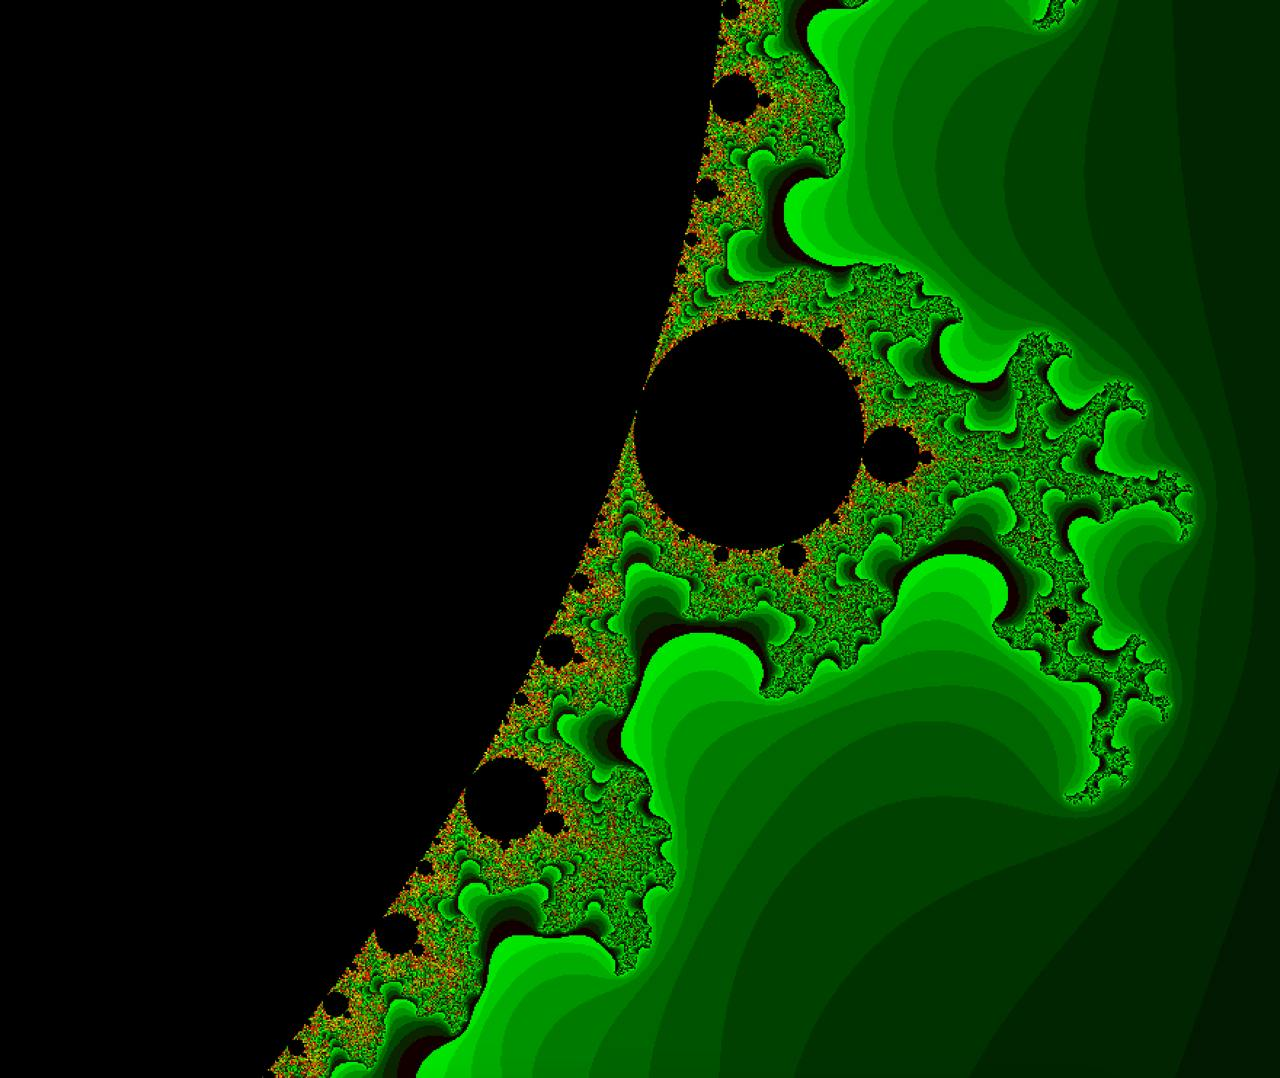
\includegraphics[width=0.5\linewidth]{mandelbroth.jpg}
   \caption{Изображение множества Мандельброта}
   \label{fig:enter-label}
\end{figure}
\begin{figure}
   \centering
   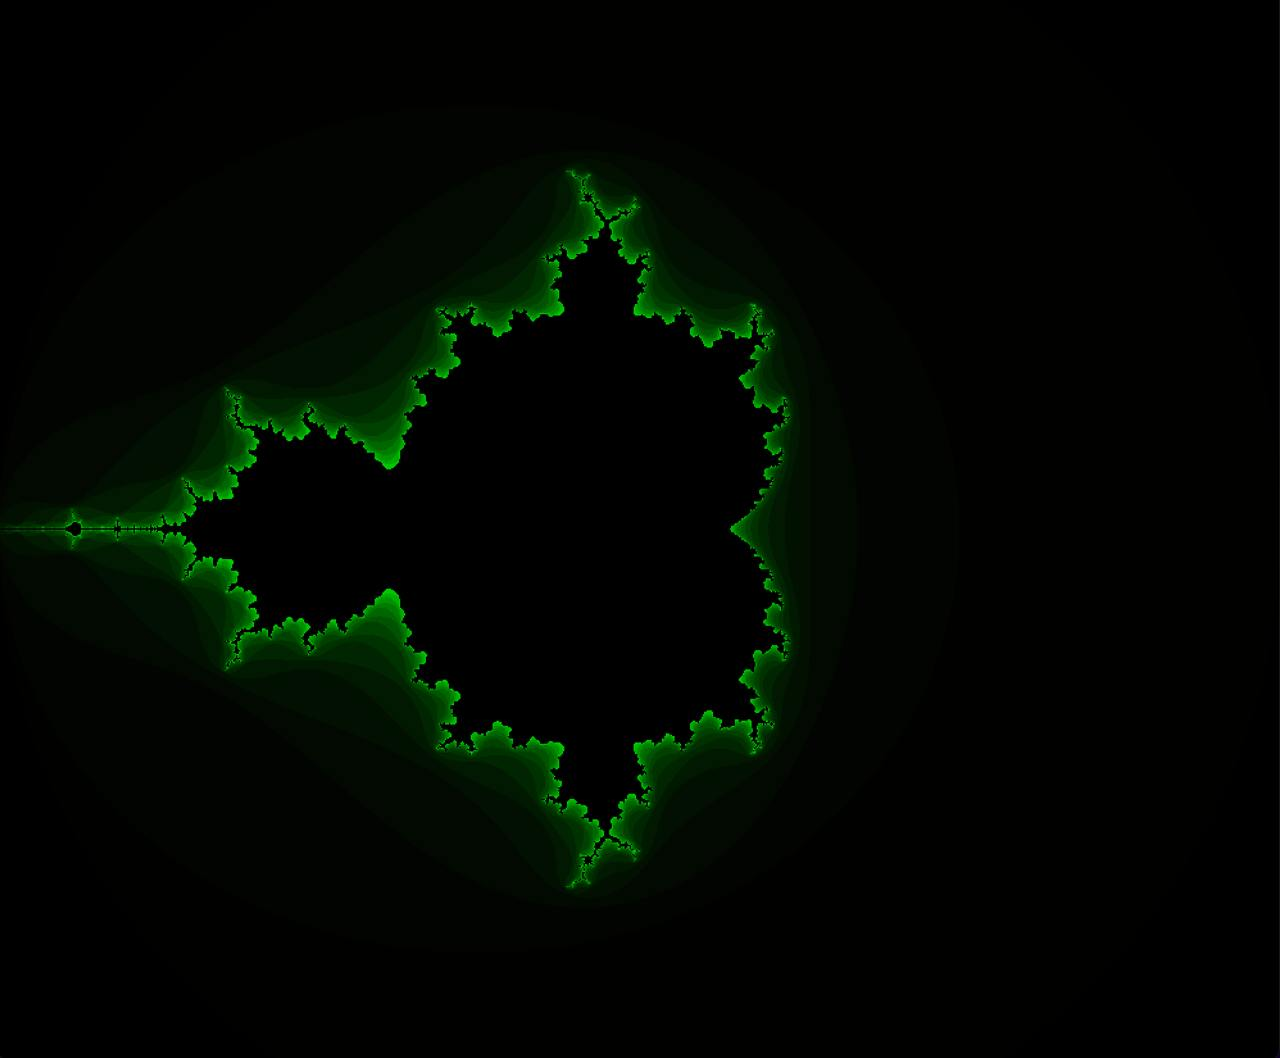
\includegraphics[width=0.5\linewidth]{m15.jpg}
   \caption{Изображение множества Мандельброта(количество итераций: 15}
   \label{fig:enter-label}
\end{figure}
\begin{figure}
   \centering
   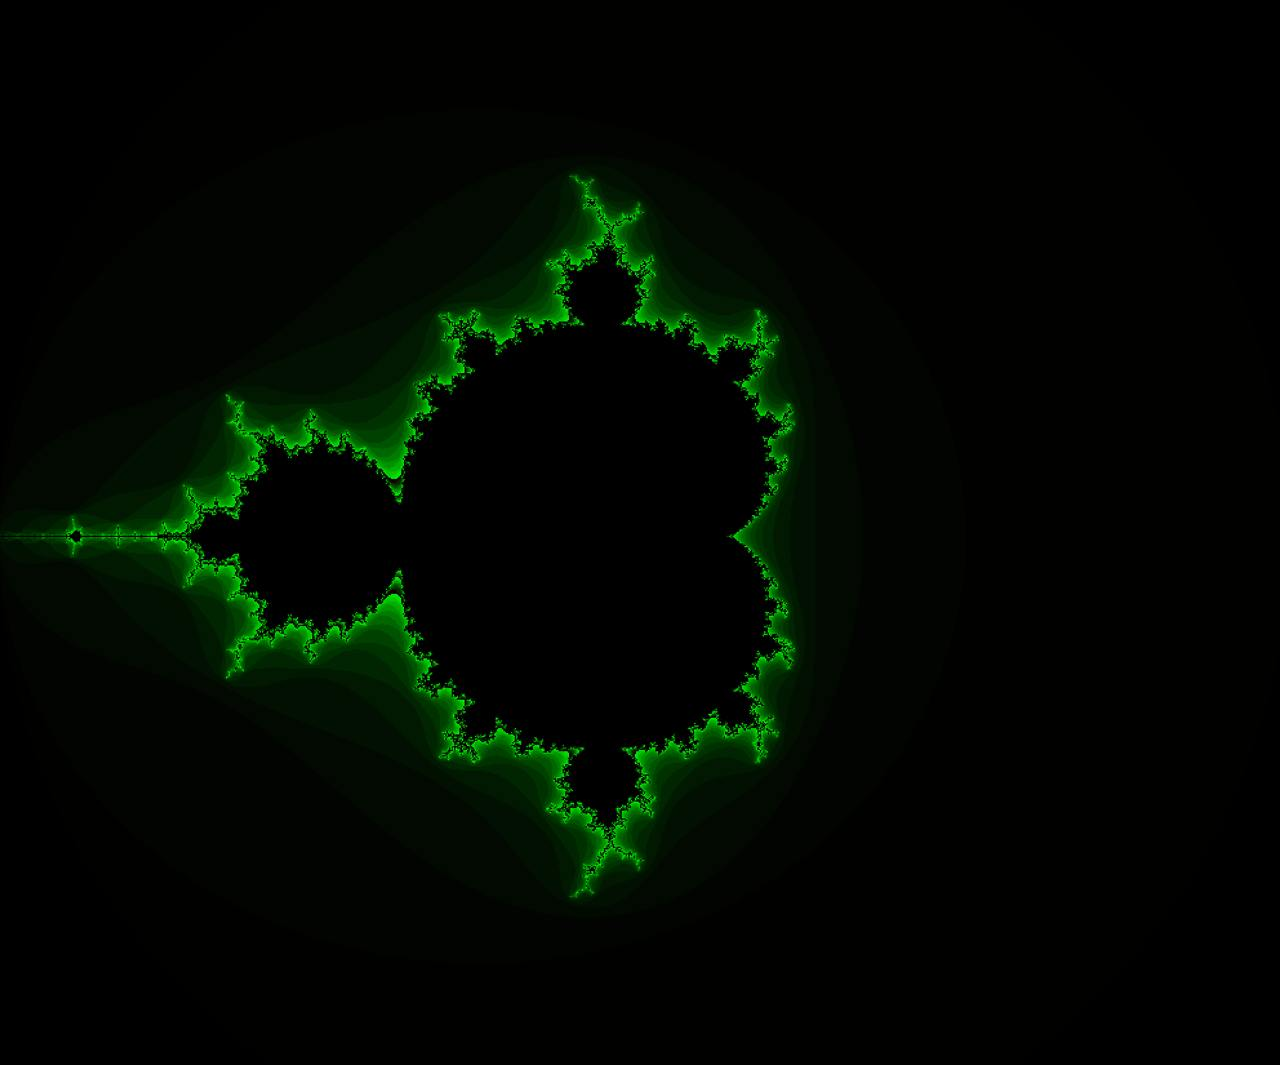
\includegraphics[width=0.5\linewidth]{m30.jpg}
   \caption{Изображение множества Мандельброта(количество итераций: 30)}
   \label{fig:enter-label}
\end{figure}
\begin{figure}
   \centering
   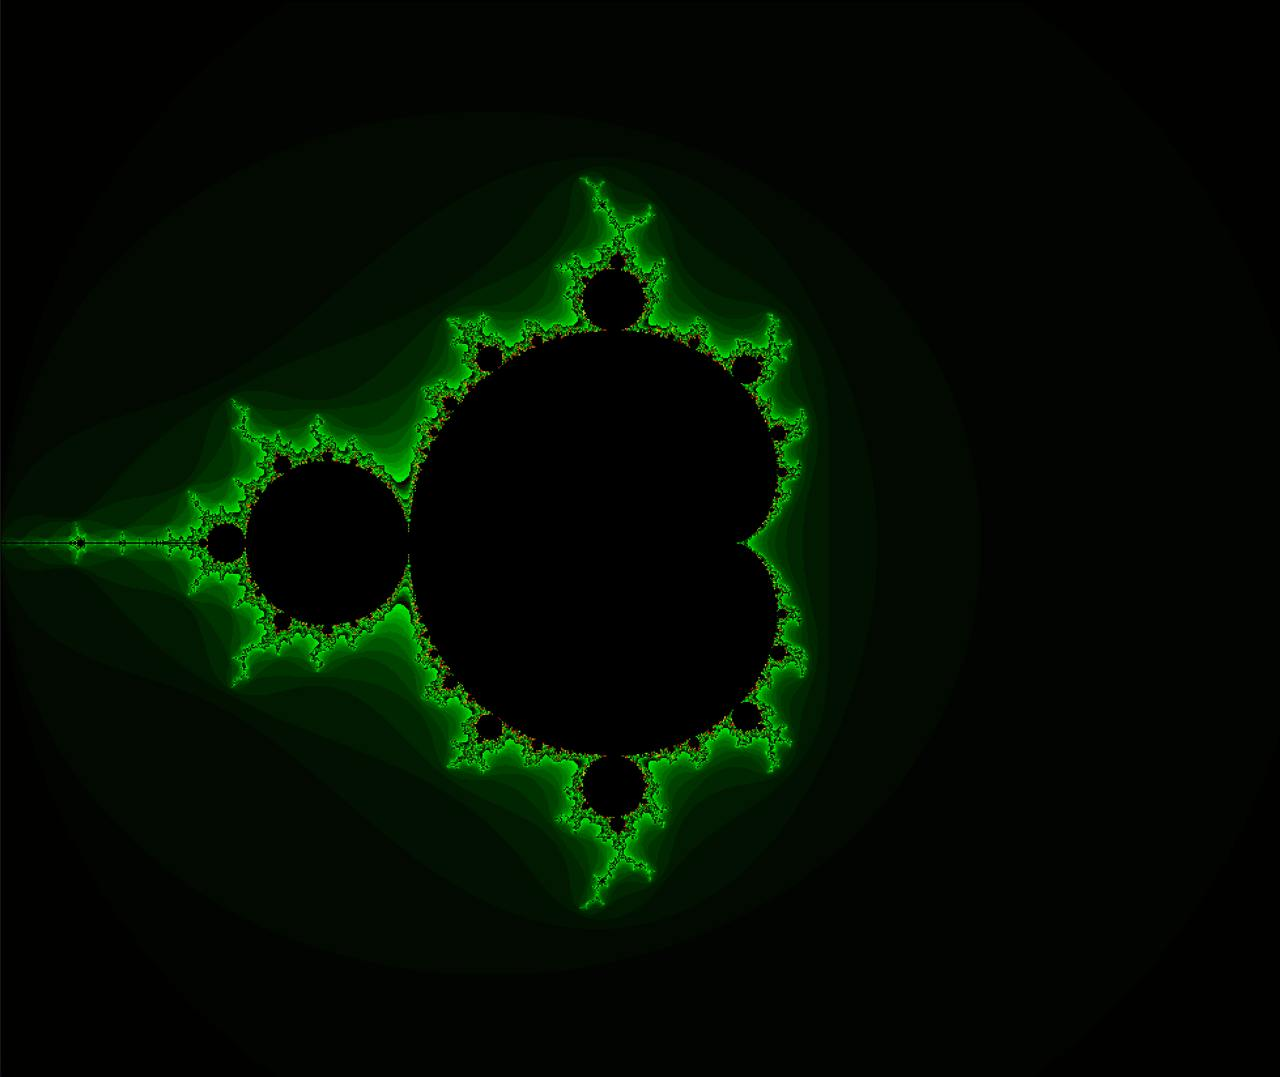
\includegraphics[width=0.5\linewidth]{m255.jpg}
   \caption{Изображение множества Мандельброта(количество итераций: 255)}
   \label{fig:enter-label}
\end{figure}
\begin{figure}
   \centering
   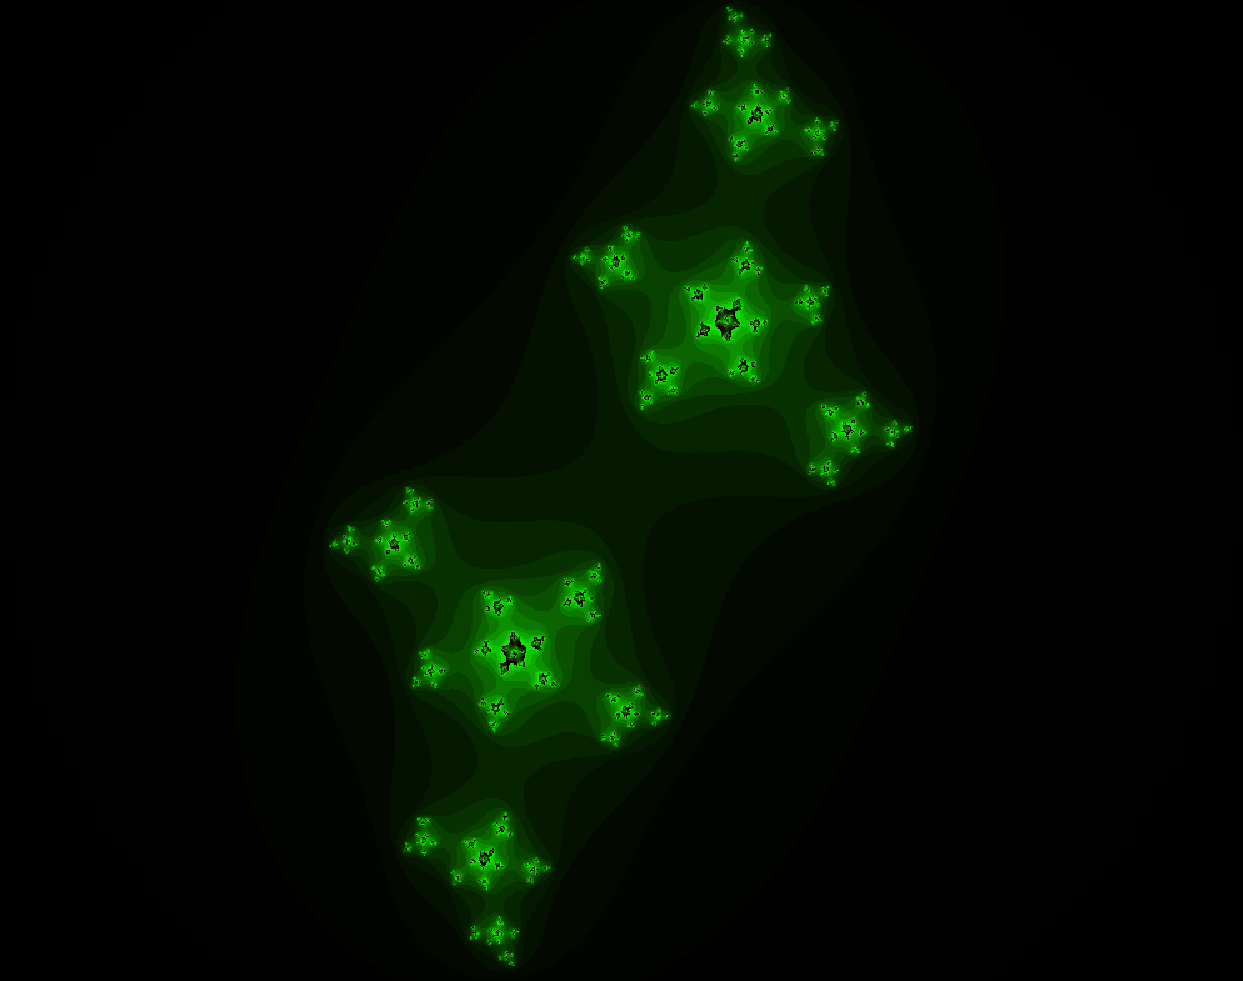
\includegraphics[width=0.5\linewidth]{julia.png}
   \caption{Изображение множества Жюлиа}
   \label{fig:enter-label}
\end{figure}
\begin{figure}
   \centering
   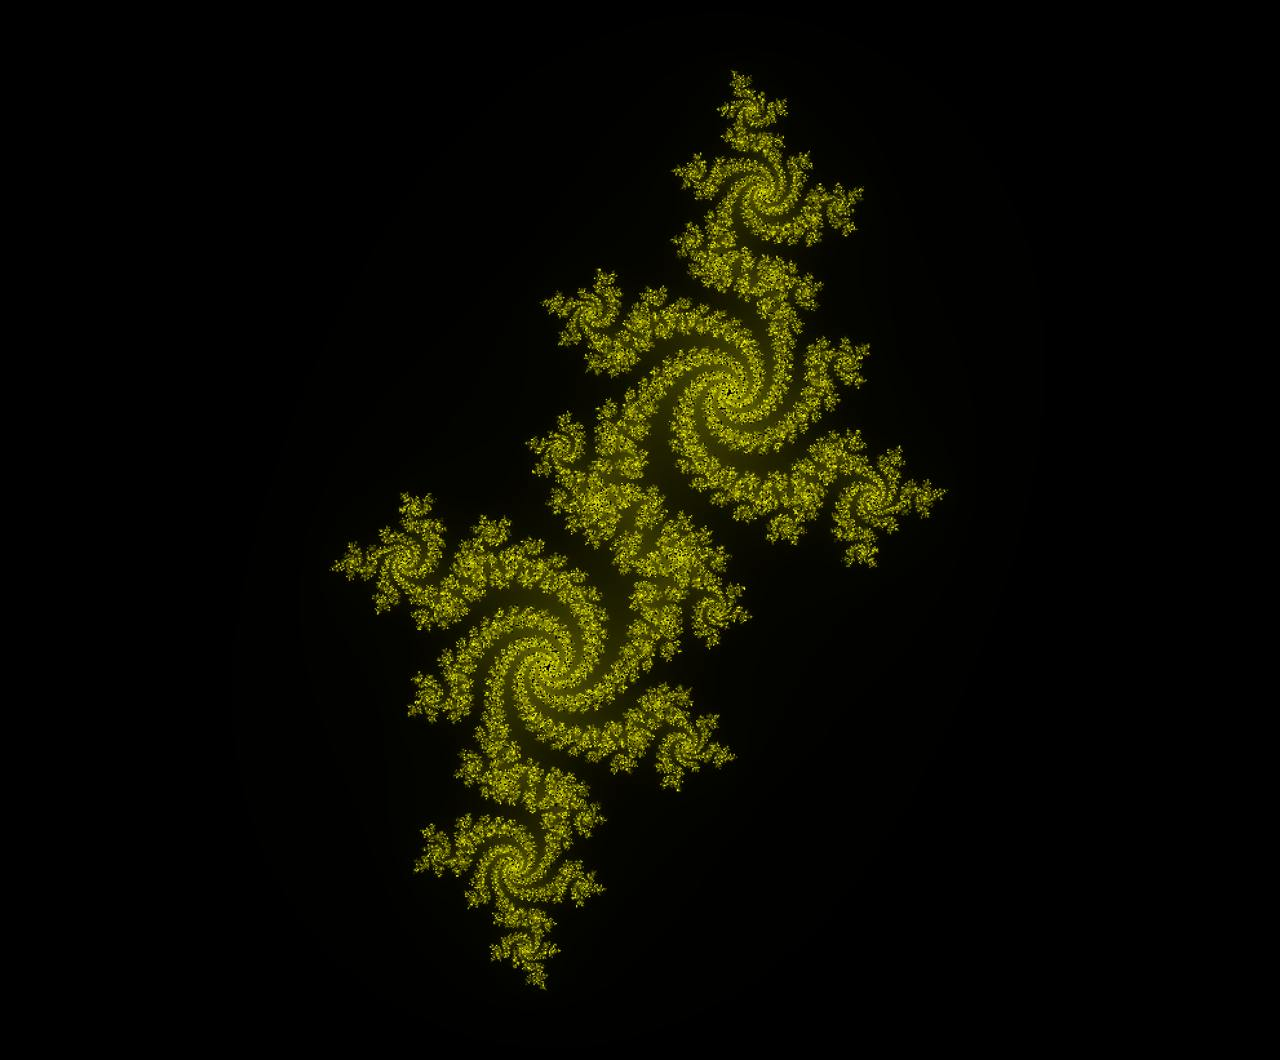
\includegraphics[width=0.5\linewidth]{j255.jpg}
   \caption{Изображение множества Жюлиа в точке ($c=−0.5251993 + i0.5251993$) (255 итераций)}
   \label{fig:enter-label}
\end{figure}
\begin{figure}
   \centering
   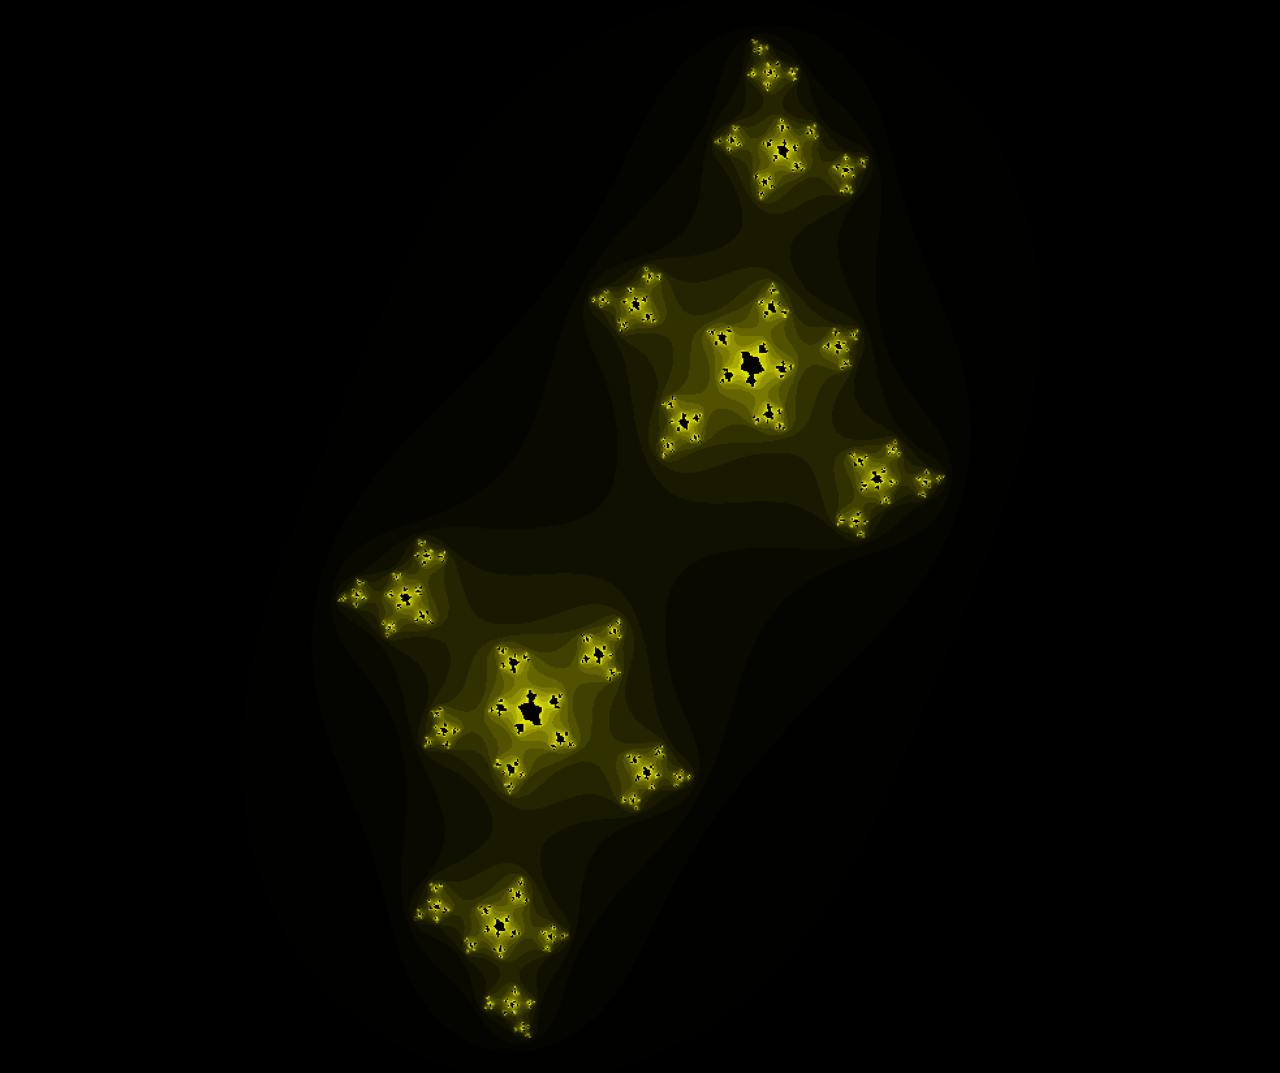
\includegraphics[width=0.5\linewidth]{j-16.jpg}
   \caption{Изображение множества Жюлиа в точке (-0.5, 0.5) (16 итераций)}
   \label{fig:enter-label}
\end{figure}
\begin{figure}
   \centering
   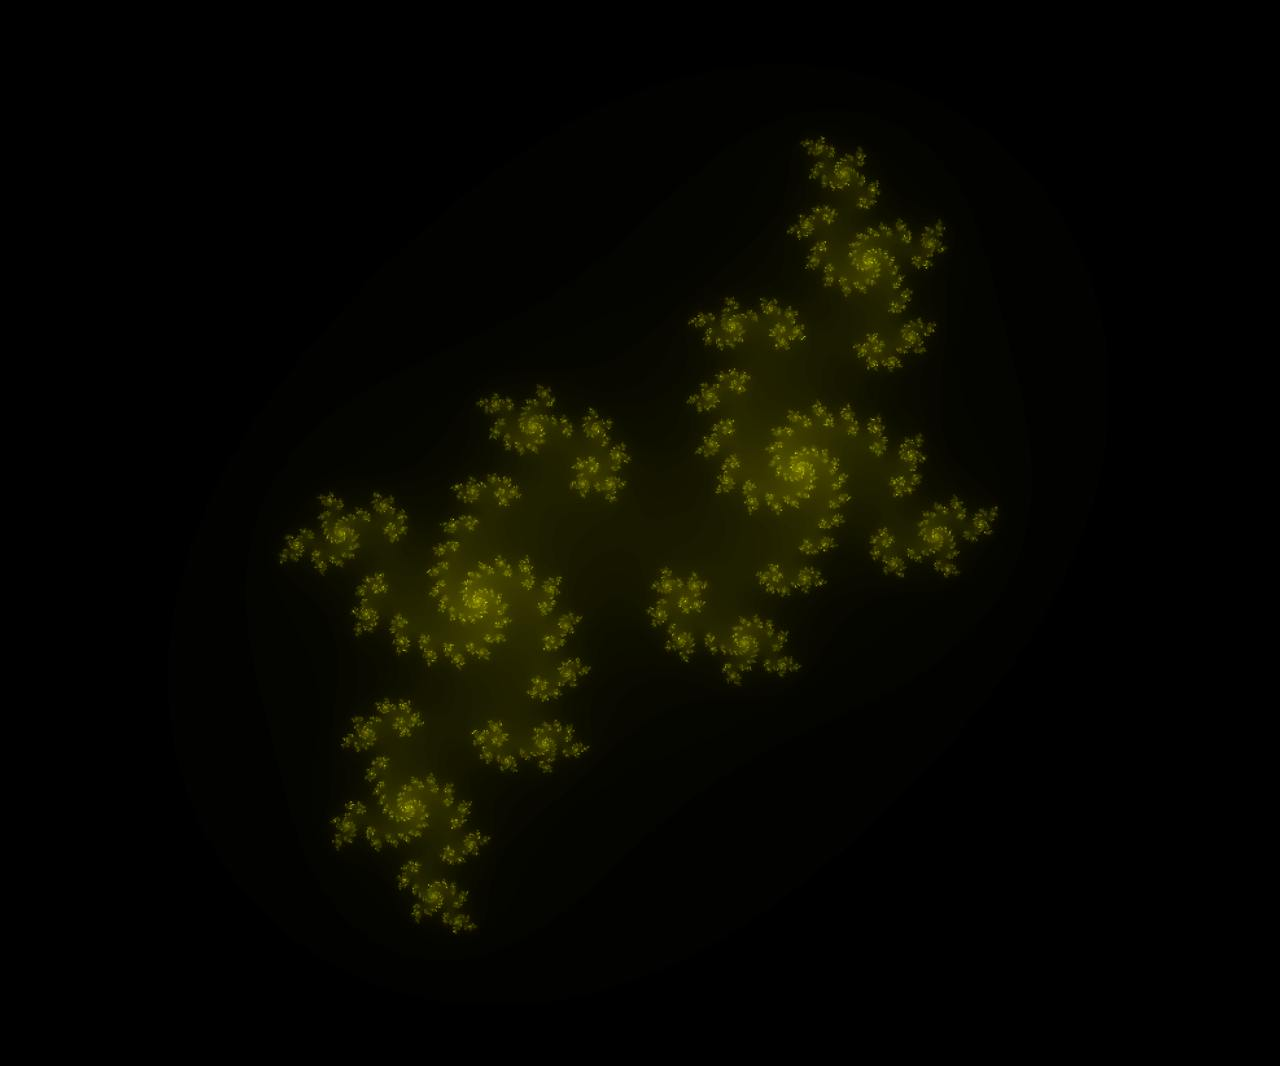
\includegraphics[width=0.5\linewidth]{j7255.jpg}
   \caption{Изображение множества Жюлиа в точке (0, 0.7) (255 итераций)}
   \label{fig:enter-label}
\end{figure}
\begin{figure}
   \centering
   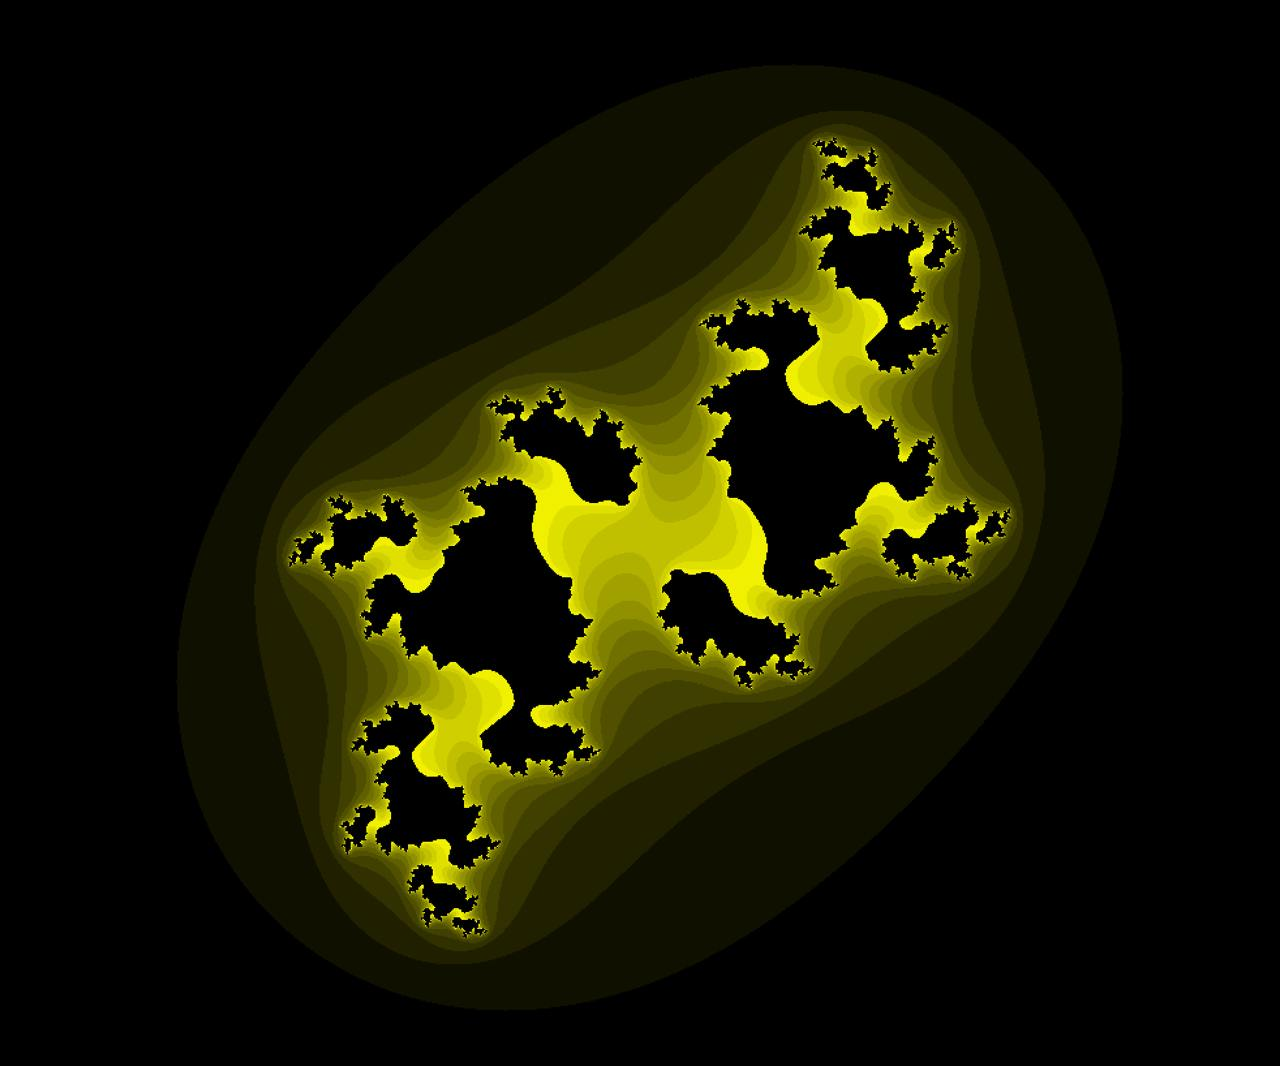
\includegraphics[width=0.5\linewidth]{j716.jpg}
   \caption{Изображение множества Жюлиа в точке (0, 0.7) (16 итераций)}
   \label{fig:enter-label}
\end{figure}
\begin{figure}
   \centering
   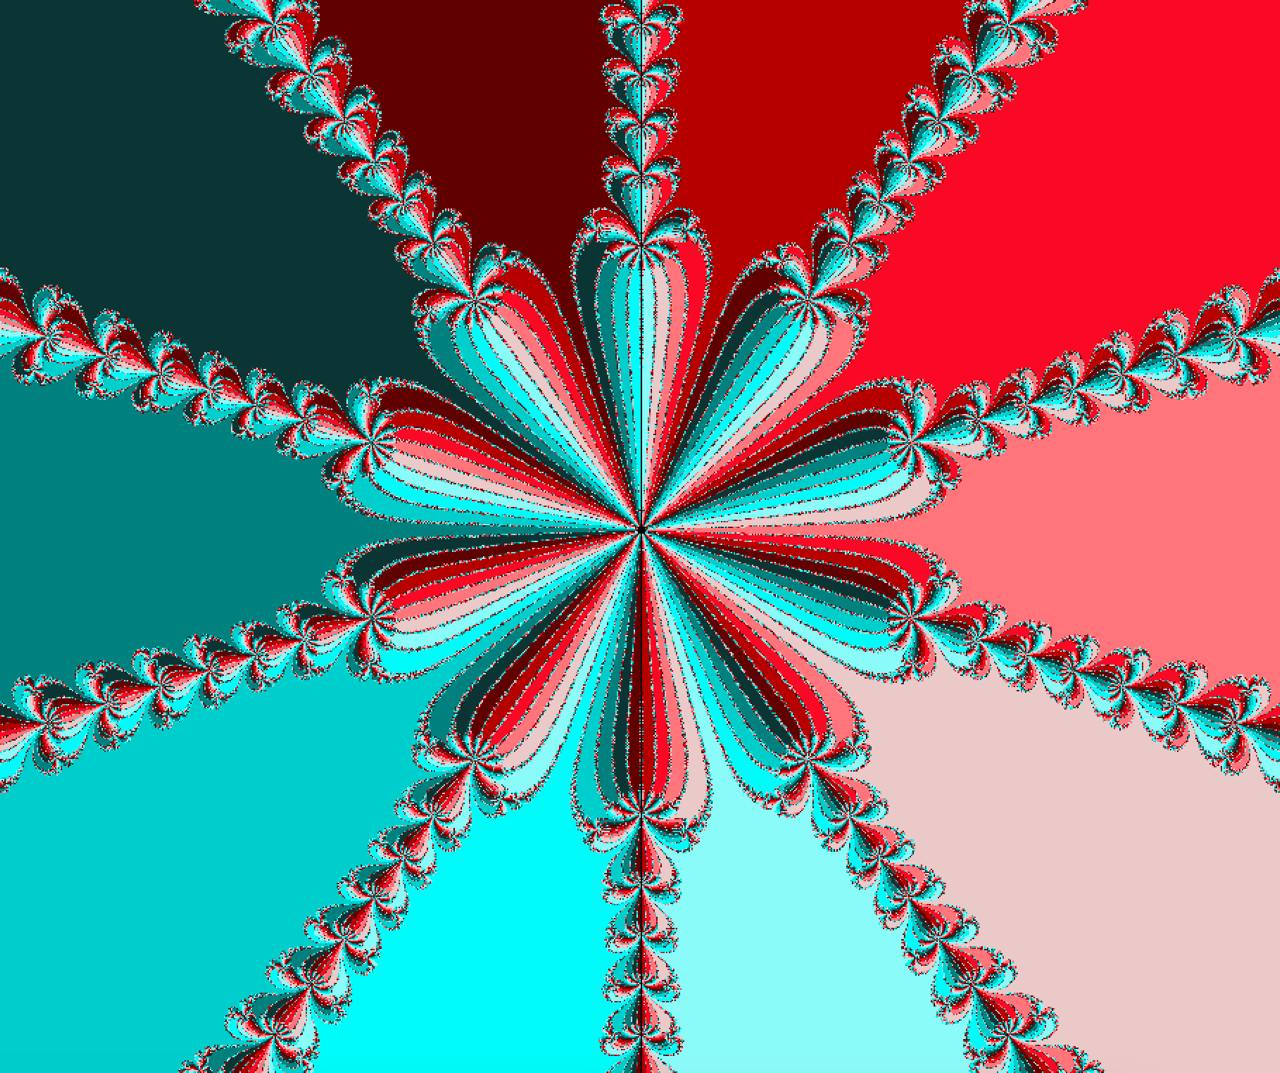
\includegraphics[width=0.5\linewidth]{newton.jpg}
   \caption{Изображение бассейнов Ньютона для многочлена $z^10 - 1$ (1000 итераций) с приближением $0.000000001$}
   \label{fig:enter-label}
\end{figure}
\begin{figure}
   \centering
   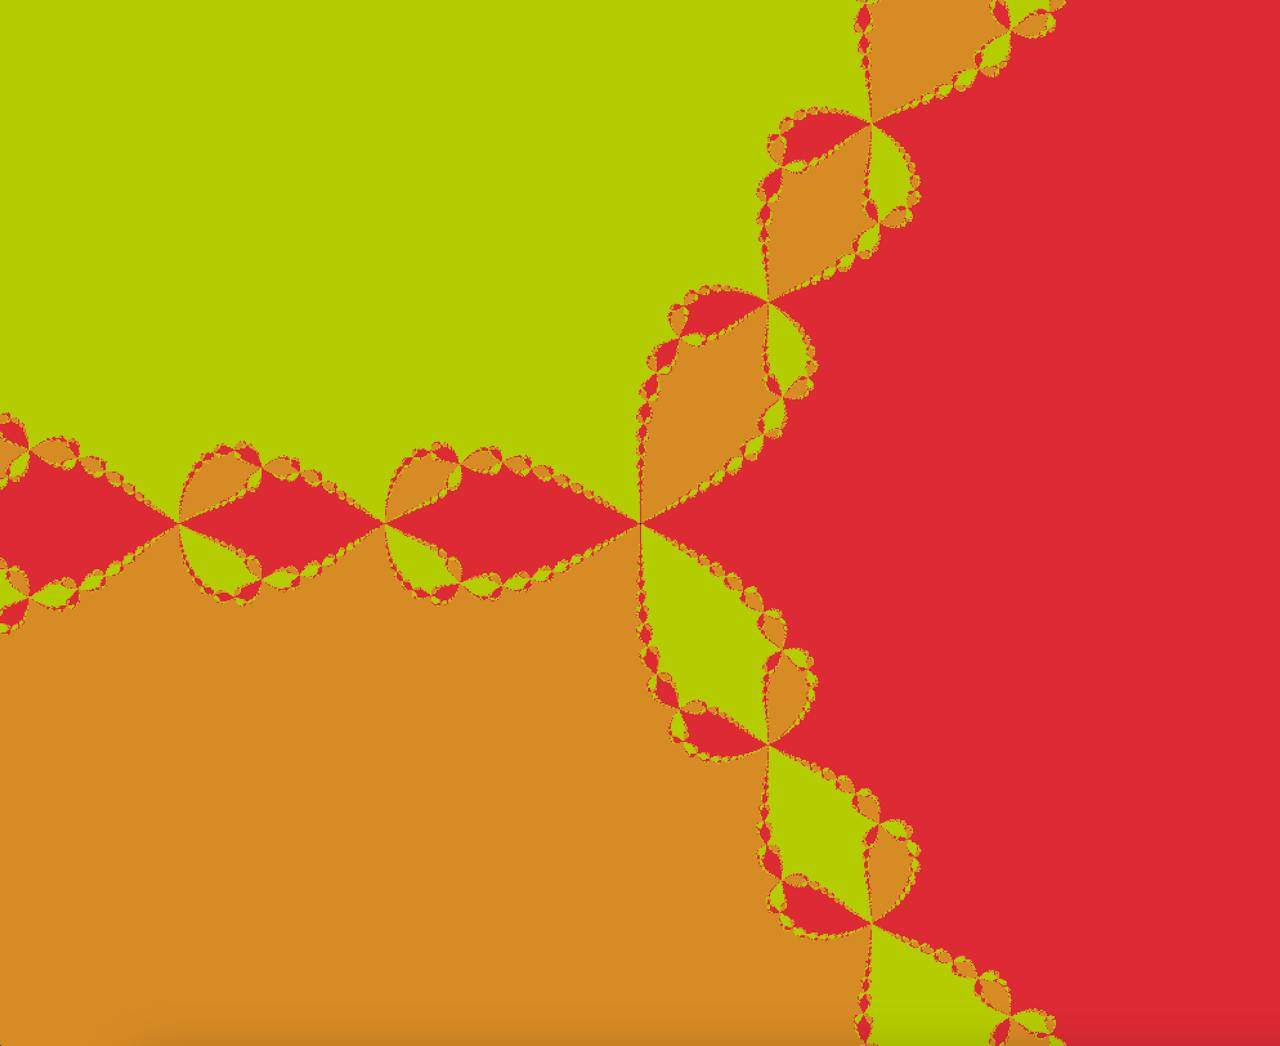
\includegraphics[width=0.5\linewidth]{n3.jpg}
   \caption{Изображение бассейнов Ньютона для многочлена $z^3 - 1$ (1000 итераций) с приближением $0.000000001$}
   \label{fig:enter-label}
\end{figure}
\begin{figure}
   \centering
   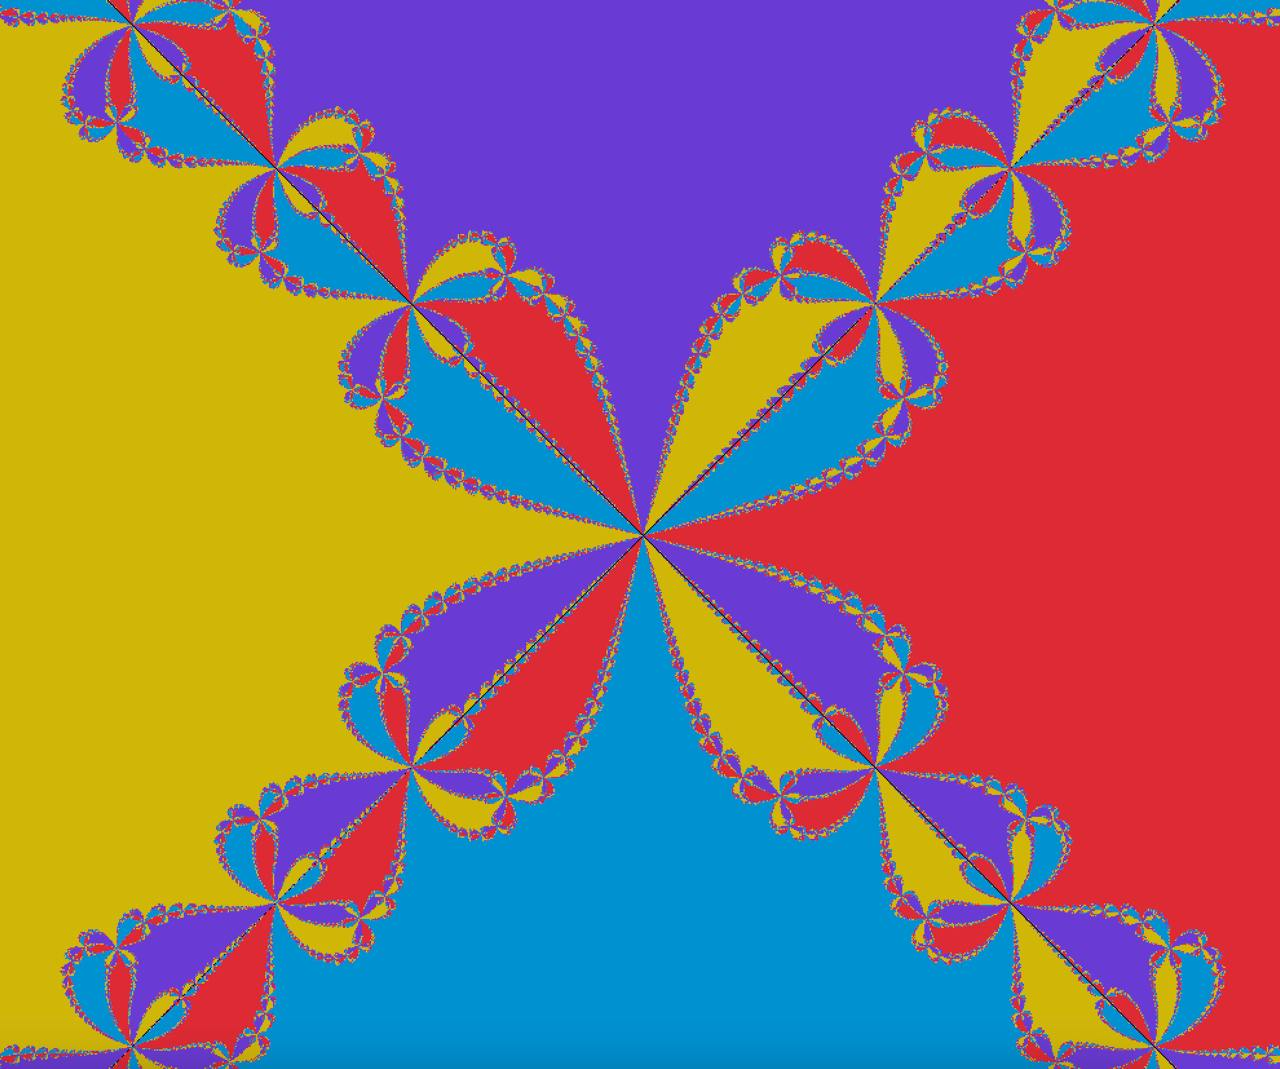
\includegraphics[width=0.5\linewidth]{n4.jpg}
   \caption{Изображение бассейнов Ньютона для многочлена $z^4 - 1$ (1000 итераций) с приближением $0.000000001$}
   \label{fig:enter-label}
\end{figure}
\end{document}
